%!TEX root = ../thesis.tex

\cleardoublepage
\chapter{Evaluation}
\label{cha:evaluation}

This chapter looks at the set-up for the experiments and presents and discusses the results achieved. In section \ref{sec:testing} the environment in which the agents were tested is explained and then in the section \ref{sec:analysis} the results are analyzed. 

\section{Testing the Agents}
\label{sec:testing}

In order to evaluate the performance of these agents they were tested on a 32-core, 125GB RAM machine against 5 different workflows from the popular bioinformatics framework nf-core \footnote{https://nf-co.re/}. Each workflow is first run 10 times without any reinforcement learning agents active. This was done primarily to have data to compare with the results later on but also so that there was historical data about the average execution time of each of the tasks, since the reinforcement learning agents need this information. After that the agents are tested. The gradient bandits are run 50 times for each workflow and the q-learning agent 100 times. As has been explained in \ref{subsub:states} the q-learning agent needs considerably longer to explore its extensive state-action space and as such needs to be trained for longer. However even though it is run twice as many times as the gradient bandit, the q-learning agent is still perhaps under-trained since the state-action space it needs to explore is so much larger than the action-space which the gradient bandit explores.

The five workflows used are the following: 1) \textit{eager} - a pipeline for genomic NGS sequencing data, 2) \textit{mhcquant} - a workflow for quantitative processing of data dependent (DDA) peptidomics data, 3) \textit{nanoseq} - which is an analysis pipeline for Nanopore DNA/RNA sequencing data, 4) \textit{viralrecon}- which can be  used to perform assembly and intra-host/low-frequency variant calling for viral sample, and 5)  \textit{metaboigniter} - a pipeline for pre-processing of mass spectrometry-based metabolomics data. 

The input data used for the workflows is based on custom combinations of different input files provided by the workflow's maintainers. For each pipeline nf-core provides full example datasets and short example datasets as well as resource configurations for each of them. The short datasets are all configured to only assign either 1 or 2 CPUs and are thus are not really feasible for comparison, however the full datasets, whilst featuring realistic configurations, often take far too long to run. For reference, the full datasets will often take 6 hours or more to run to completion whereas the short examples never take more than 5 minutes. 

In order to build pipelines with more realistic runtimes, configurations and input data, but without running too long, the short examples and the full ones need to be combined. The combinations are designed to strike a balance between having large input data and realistic task configurations but also being short enough that it is feasible to run the workflows tens or even hundreds of times. Each workflow’s set of inputs is built individually by following the same overarching tactic. First, start with the command line arguments from the short datasets (these sometimes omit certain steps which can speed up execution) and then combine those with the configuration and the input data from the full dataset. After this the input files are reduced until the pipeline completes in a reasonable amount of time. As an example, one of the genome sequencing workflows was sequencing several different genomes, so to speed up execution but keep realistic data the number of genomes to be sequenced was changed to one by removing input files containing the other genomes. By following this process, configurations and inputs were found for all five of the pipelines mentioned above such that they were completing after around 10 to 40 minutes.  

Nextflow inherently keeps track of the total number of resources available and the resources already assigned to tasks and it will not schedule more resources than the system has left. The tasks are all run inside of docker containers with the exact amount of CPUs and memory requested by the task. Since the tasks are all being run on the same machine it would have been possible to ignore the sum of the resource requests and over-assign resources so that all of the tasks compete with each other, but this does not reflect situations where pipelines are being run on clusters with resource managers, and as such this was left unchanged.

For the final comparison in the next section the last 10 runs of each of the agents are compared with the 10 runs with the default configurations and 10 runs using a feedback loop approach. The feedback loop approach functions as follows: first, during training, the workflows are run 10 times and each task is assigned the maximum number of CPUs and memory available. Then, in the next 10 runs the task are assigned the average number of CPUs used during the training and the mean plus the standard deviation of the amount of memory used . Should a task fail, then it is retried with the maximum amount of memory ever used by that task during the training time, and should it fail again then it is retried with double that value. This feedback loop approach has been mentioned in chapter \ref{cha:related_work} and it is based on the work from \cite{tovarjob} and \cite{FeedbackBasedAllocation}.



%%=========================================
\section{Results and Discussion}
\label{sec:analysis}

\subsection{Performance Comparison}
\label{sub:comp_perf}

\begin{figure}[h]
    \centering
        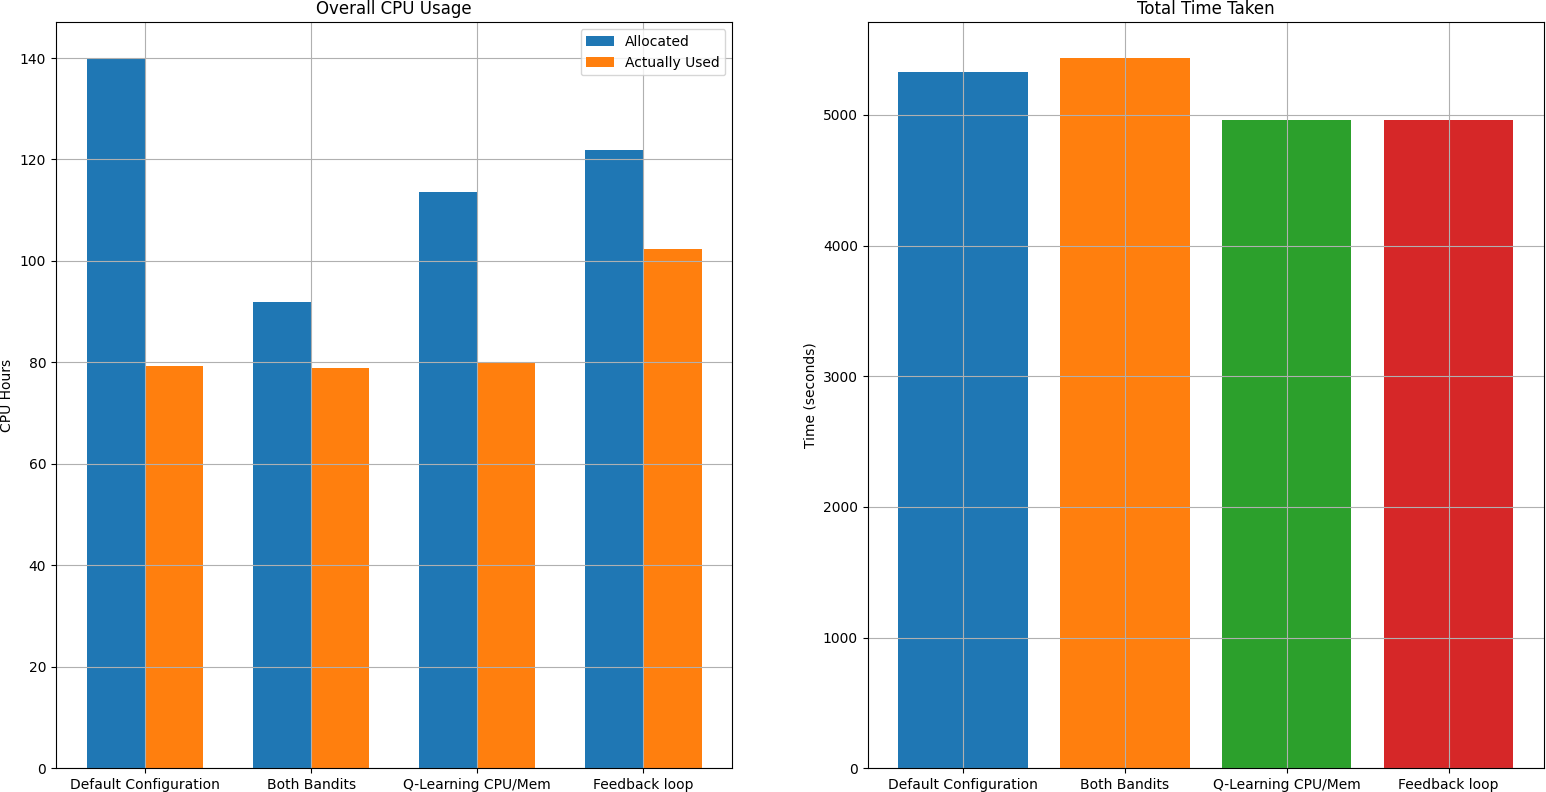
\includegraphics[width=\textwidth]{fig/cpu_mem_results.png}
        \caption{Performance of the CPU and Memory Approaches}
        \label{fig:cpu_results}
\end{figure}

\begin{figure}[h]
    \centering
        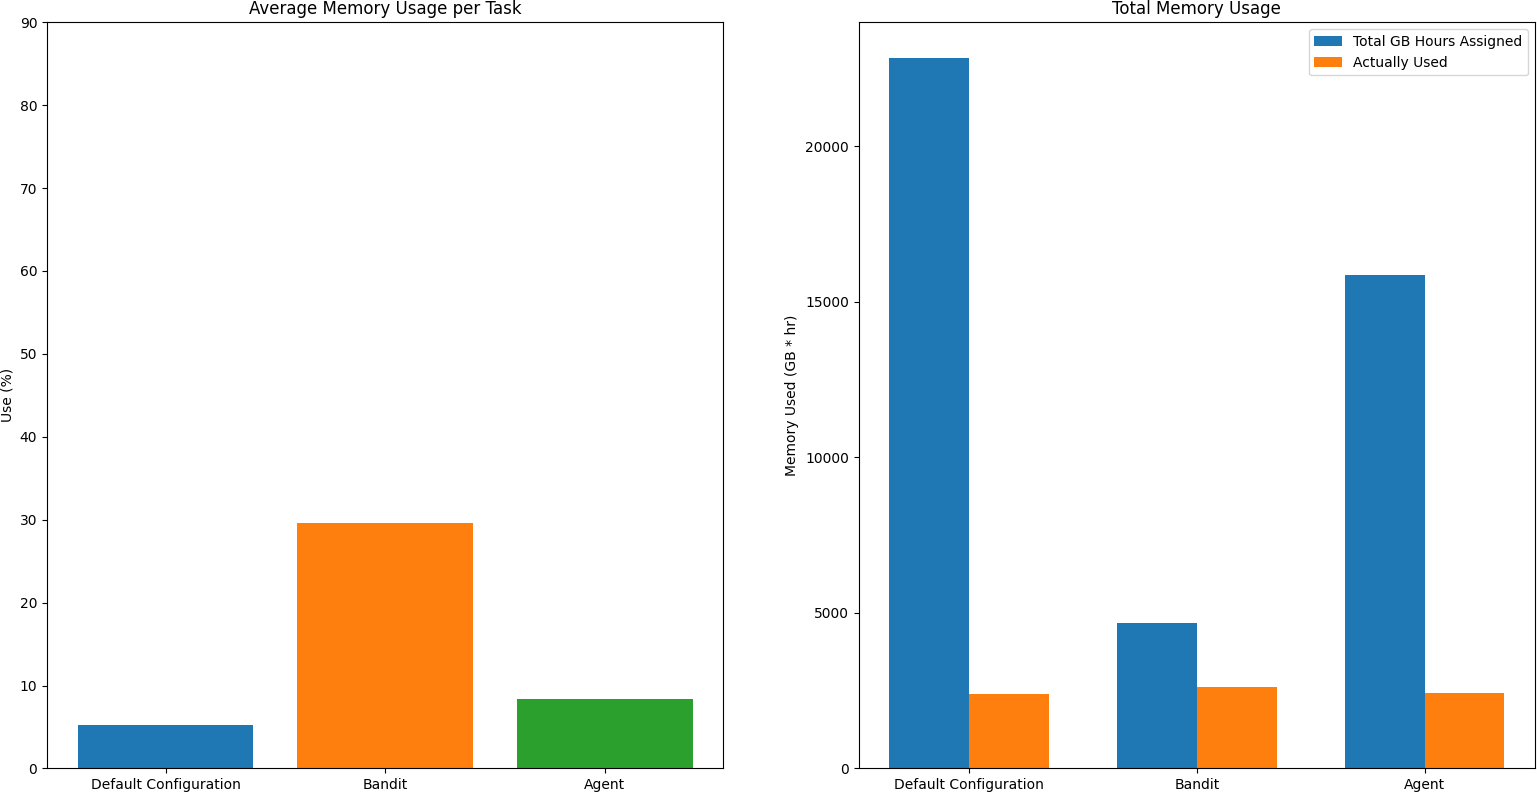
\includegraphics[width=\textwidth]{fig/cropped_memory_usage_final.png}
        \caption{Memory Usage}
        \label{fig:mem_use}
\end{figure}

In this section the performance of the gradient bandit, the q-learning approach, the default configuration and the feedback loop will be compared. All of these comparison are for 10 runs of each of the 5 workflows, for the q-learning and gradient bandit approaches only their last 10 runs of each workflow are considered.

Figures \ref{fig:cpu_results} and \ref{fig:mem_use} show how these approaches performed. The left graph in the first figure shows the total amount of CPU hours used by all of the tasks across all of the workflows and the amount of CPU hours that were actually used (also called the effective CPU hours). Effective CPU hours are the CPU usage multiplied by the execution time whereas the CPU hours are just the number of CPUs assigned multiplied by the execution time. For example a task which was assigned 3 CPUs, ran for 1 hour and had 200\% CPU usage would have used 3 CPU hours but only 2 effective CPU hours. These values are calculated for each individual task and then summed up over all of the workflows.

The right graph in the first figure (\ref{fig:cpu_results}) shows the cumulative amount of time it took for all of the workflows to run to completion. In the second figure, \ref{fig:mem_use}, the memory usage is shown. The unit measured in the right graph of \ref{fig:mem_use} is the gigabyte hour and the graph displays the total amount of gigabyte hours allocated across all of the workflows as well as the actual amount of gigabyte hours used (based on each task’s peak RSS and execution time- this is the minimum amount of gigabyte hours which could have been assigned without the task being killed). The left graph of that figure shows the average memory usage across all of the tasks, where memory usage is the task’s peak RSS value divided by the total memory assigned to it. 

From these graphs it is clear to see that all of the reinforcement learning approaches managed to improve CPU efficiency and allocate less CPU hours than the default configuration. In the case of the gradient bandit it was particularly effective at keeping the overall CPU hours assigned to an absolute minimum, however it seems that this efficiency came at the cost of speed, and it performed worse than its q-learning counterpart in this aspect and took slightly longer than the default configuration. The q-learning approach was faster than the default configuration and was more efficient with regards to CPU usage. As can be seen, both of the reinforcement learning approaches are able to assign less CPU hours without having a detrimental effect on execution time (in fact the q-learning approach assigns less CPU hours but executes faster). Looking at the reward function of the q-learning agent (\ref{q_agent_1_reward}), the “CPU usage”considered by the function is not the task’s actual usage but rather the maximum of either 90 or the CPU usage. As such agents for tasks which exhibit very high CPU usage ($>90\%$) receive no additional reward for increased efficiency (since efficiency can always be increased by decreasing the total number of CPUs assigned) so their rewards depend entirely on the execution time and they are thus encouraged to find resource allocations which decrease runtime. This most likely explains why the gradient bandit is more efficient but the q-learning agent is faster.

When compared with the feedback loop, the gradient bandit is 11\% slower but uses 25\% less CPU hours, whilst the q-learning agent performs worse in every aspect except for execution time (it was only 0.03\% slower). Ultimately the fact that the feedback loop approach assigns less CPU hours than the q-learning agent but is still marginally faster indicates that the q-learning approach has not found the right balance between increased resource usage at the cost of faster execution, however the fact that the gradient bandits assigned percentually less CPU hours than the percentage by which it was slower than the feedback loop indicates it is able to trade off reduced execution times for more efficient CPU allocations.

Interestingly, the feedback loop increased the effective CPU hours used by the workflows, something which had remained constant under the other 3 configurations, and the feedback loop approach was actually quite efficient in terms of the total amount of CPU hours assigned relative to the increased effective usage. It can only be speculated as to why it used more actual CPU hours than the other approaches but it may be down to the fact that certain highly parallelizable tasks will be assigned incredibly large numbers of CPUs, far beyond the point of diminishing returns, and eventually lead to the workflow using more effective CPU hours (as an example one task recorded 2800\% CPU usage during training and as such was assigned 28 CPUs by the feedback loop). This would indicate that assigning more resources may actually increase their usage, something which the feedback loop approach assumes is false.

Concerning memory allocations, both of the reinforcement learning approaches proved to be better than the default configuration. One aspect which stands out is how poor the default configurations are. On average they are using just 5\% of the assigned memory. On the other hand the q-learning approach is not much more efficient, however it still reduces the wasted memory by a large amount (around 5000 gigabyte hours were saved compared to the default configuration). Yet this amount is dwarfed by the other two approaches which save close to 15000 gigabyte hours and reduce the memory assignments by 80 and 87 \% respectively. The gradient bandit approach performed better than the q-learning approach by a significant margin and it assigned less than half as many memory hours as either the default configuration or the q-learning agent. The feedback loop approach is clearly the best, assigning the least amount of memory hours overall and showing very high memory usage for all of the tasks.

Ultimately the performance of the q-learning agent is down to the fact that the number of chunks of memory it could choose from was very low (in order to have less states so that it could be trained faster), and thus it had a fairly limited extent to which it could reduce the memory usage. The gradient bandit suffers from this too because ultimately it also only had a fixed number of memory chunks to choose from and could only increase or decrease a task’s memory usage by a multiple of the size of the memory chunks. The feedback loop does not have this problem and can assign memory at the most granular level possible. It therefore follows that it would naturally be able to outperform these two approaches which can only assign chunks of memory. Another factor to consider is that both of the reinforcement learning approaches also had the option to assign more memory than the default configuration. This was clearly unnecessary, and because all of the tasks were using much less memory than the default amount it would have been possible to change the agents’ options to only be chunks of memory which added up to less than the default amount. This would have increased their performance. 

This same problem is also reflected (to an extent) in the q-learning agent’s CPU allocations, where the q-learning agent is inefficient relative to the other two approaches, because it was given a limited number of CPU allocation options to choose from in order to keep its state-action space small. 

\subsection{Performance on a Workflow by Workflow Basis}
\label{sub:per_wf}

%\begin{figure}[ht]
%\centering
%\begin{subfigure}{.5\textwidth}
% 	%\centering
%        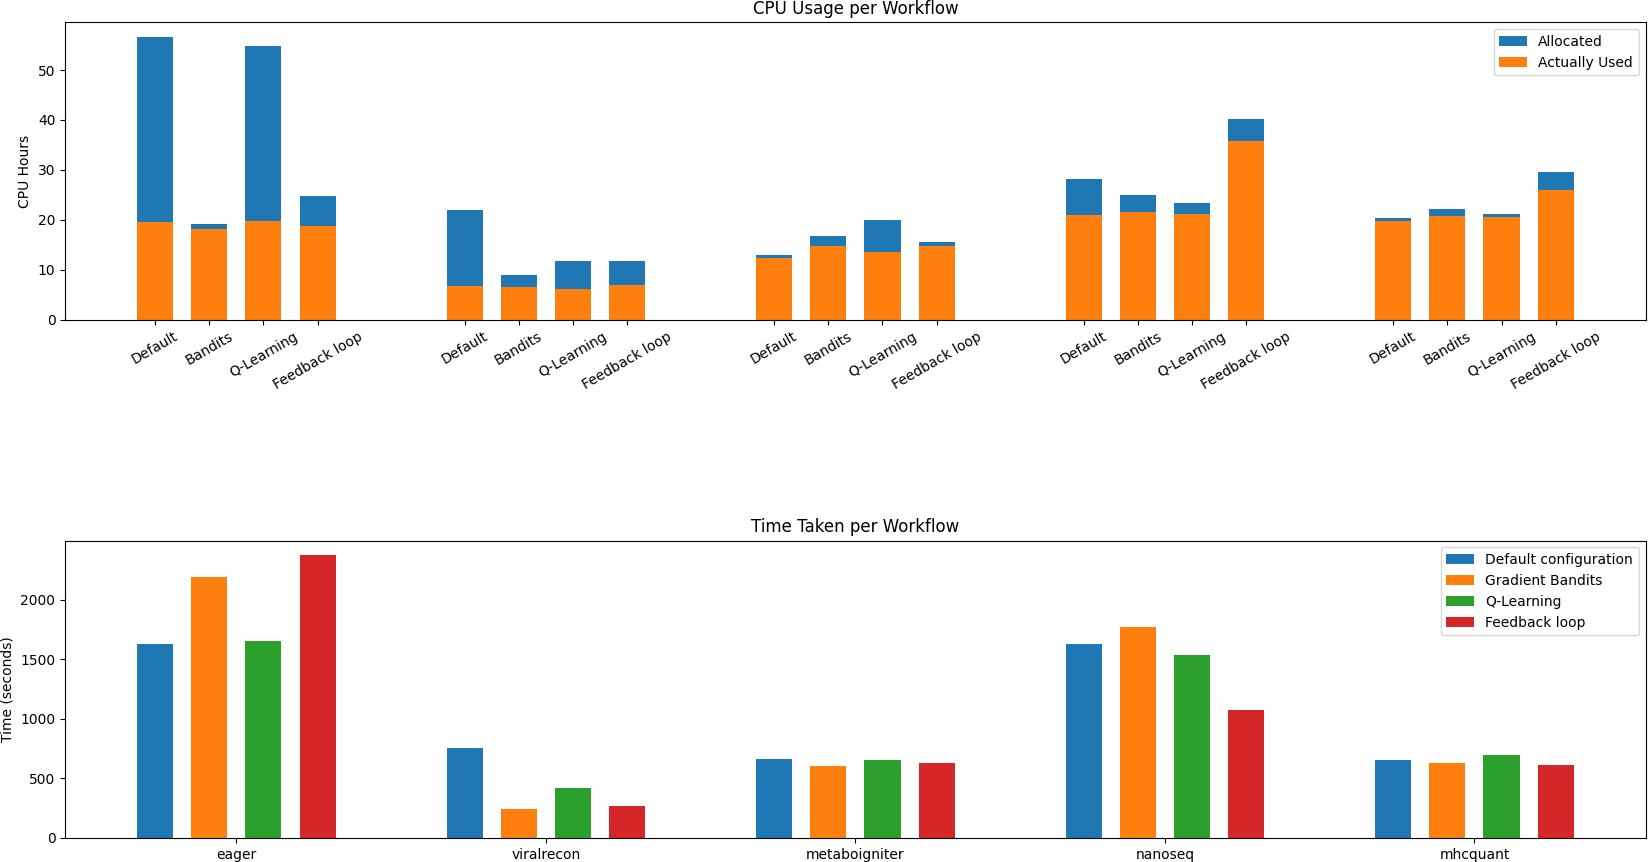
\includegraphics[width=\textwidth]{fig/per_wf_stats.png}
%        \caption{CPU and Execution Time}
%        \label{fig:per_wf_cpu}
%\end{subfigure}%
%\begin{subfigure}{.5\textwidth}
% % \centering
% 	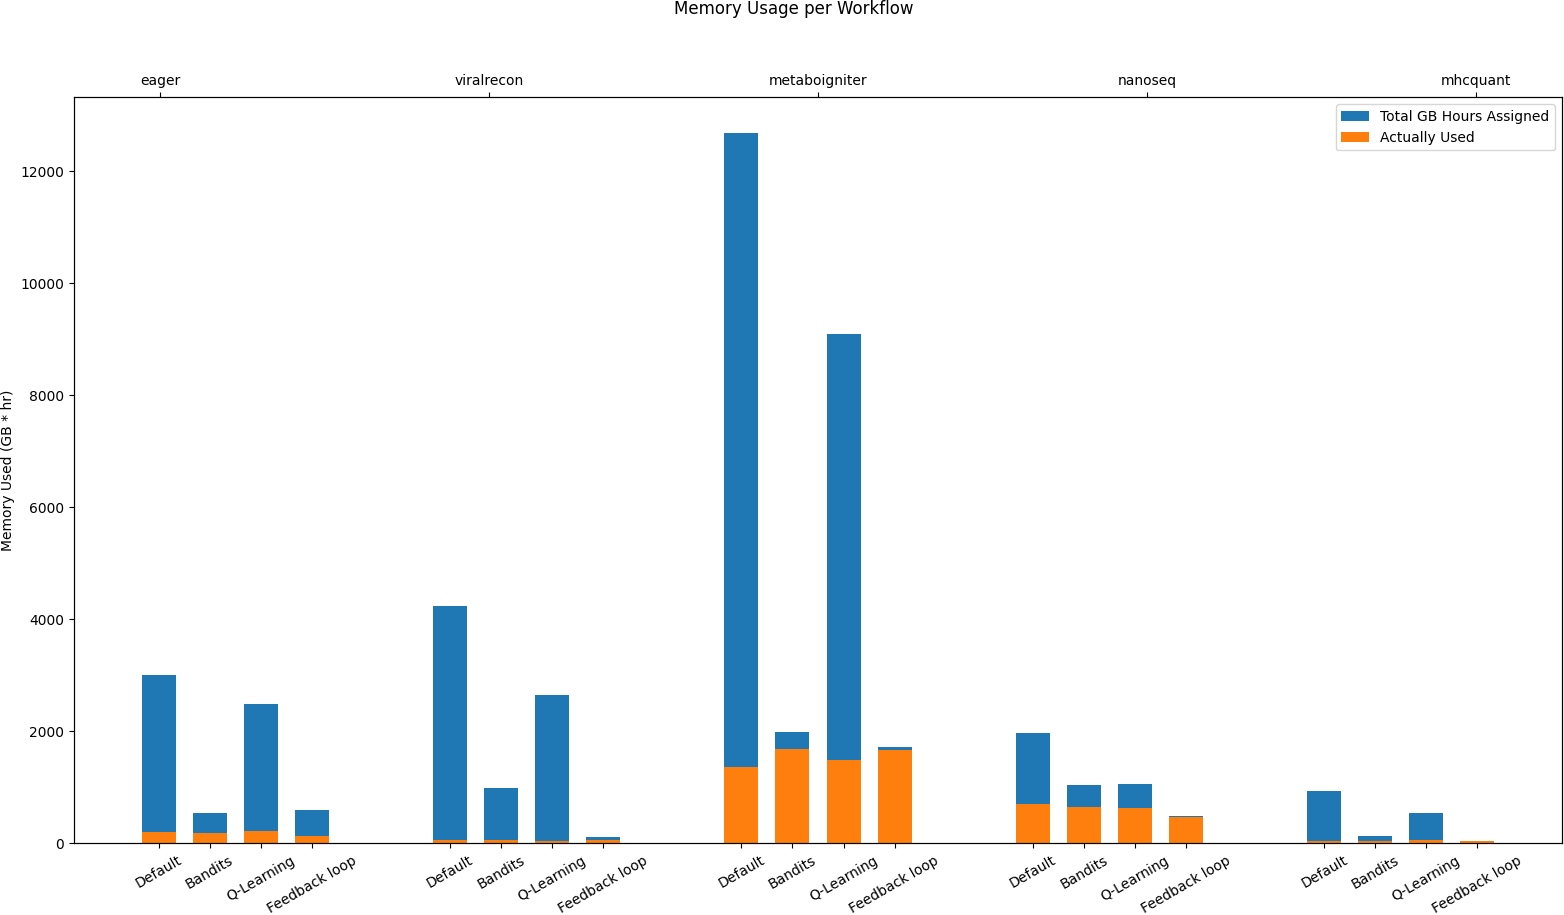
\includegraphics[width=\textwidth]{fig/mem_use_per_wf.png}
%	\caption{Memory}
%	\label{fig:per_wf_mem}
%\end{subfigure}
%\caption{Example of Two Bandits Converging Too Fast}
%%\label{fig:old_bandits}
%\end{figure}

\begin{figure}[h!]
    \centering
        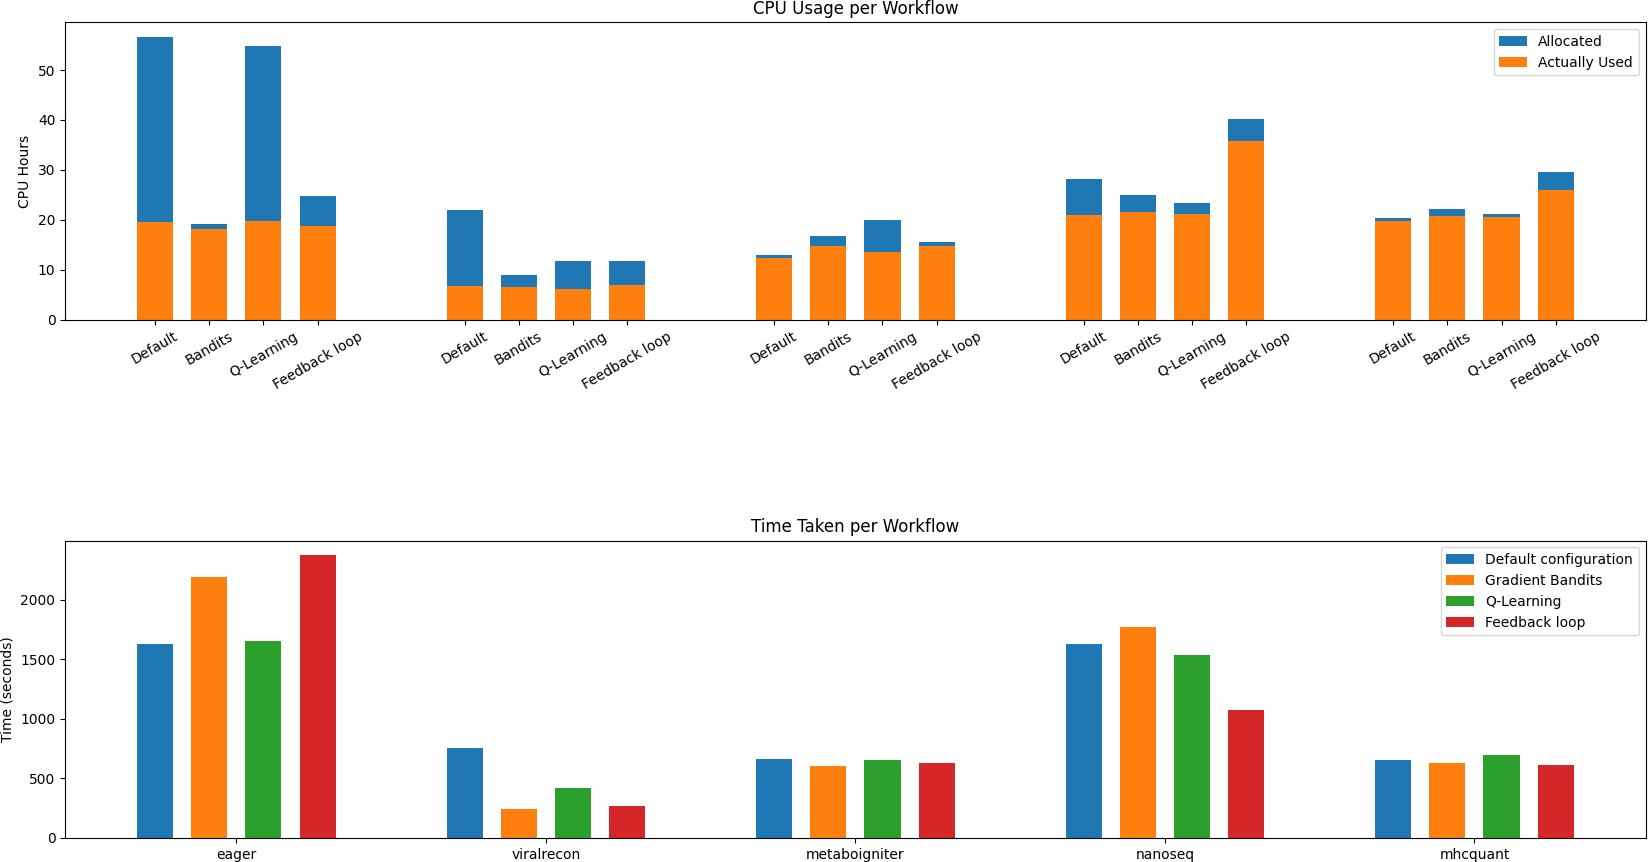
\includegraphics[width=\textwidth]{fig/per_wf_stats.png}
        \caption{CPU and Execution Time}
        \label{fig:per_wf_cpu}
\end{figure}

\begin{figure}[h!]
    \centering
        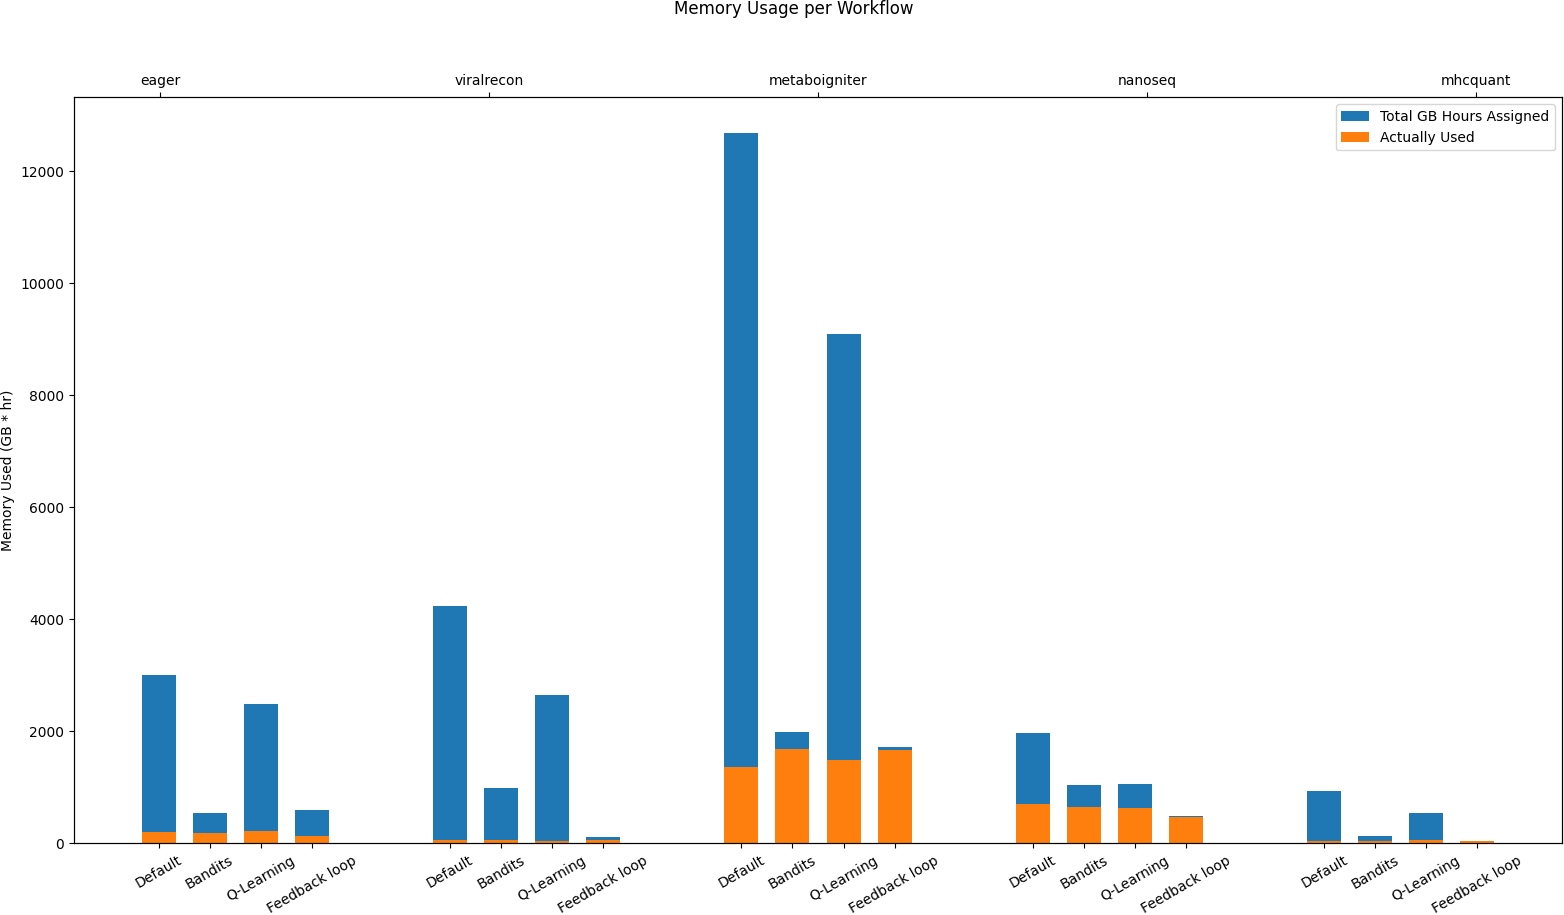
\includegraphics[width=\textwidth]{fig/mem_use_per_wf.png}
        \caption{Memory}
        \label{fig:per_wf_mem}
\end{figure}

In this section the results are shown by workflow, the first figure, \ref{fig:per_wf_cpu} shows the CPU usage and execution time in two separate graphs, with the bars grouped together by workflow and labelled with the approach. The workflows in the top graph of figure \ref{fig:per_wf_cpu} correspond to the labels in the bottom graph. The second figure, \ref{fig:per_wf_mem}, in a similar fashion, shows the memory usage.

It is quite difficult to find any outliers or patterns in this data and really the performance of the different approaches varies from one workflow to another, with each approach at one point or another being either the slowest or the fastest. Worth noting is of course the \textit{eager} workflow. While the CPU assignments and base usage are quite similar for most of the other workflows, with \textit{eager} the default configuration and the q-learning agent assign noticeably more CPU hours than are needed, however they achieve a faster execution time as a result. This indicates firstly that the authors of the workflow were most likely aware that there were tasks in this workflow which may have low CPU usage for periods of times but their execution speed still scales with more resources. Secondly this indicates that the q-learning agent was able to learn this and make the decision to assign more resources, even if the usage is low, because they decreased execution time. This is a direct result of the q-learning agent’s reward function, which is geared slightly more towards speed. Lastly it may also be the case that the tasks in this workflow are more Input/Output (I/O) intensive and that would indicate the need to account for I/O intensive tasks in the reinforcement learning approaches. Tasks with lots of I/O operations generally have lower CPU usage because they must wait for system calls to complete read and write operations but may still benefit from increased CPUs because they are quite CPU intensive during the time between I/O operations.

Beyond this it can also be seen in the \textit{nanoseq} and \textit{mhcquant} workflows that the feedback loop assigns more CPU hours than any other workflow and it’s effective usage is higher than that of the other approaches. This may indicate, as was speculated in the previous section, that these workflows contain highly parallelizable tasks whose resource usage scales with the resource assignment. This theory is supported by the fact that all 3 of the other approaches showed very high CPU usage for these workflows and they are most likely composed of very efficient tasks which will always use a large percentage of the resources assigned to them and may increase their usage when assigned more resources.

\subsection{Summary}
\label{sub:summary}

In conclusion all of the reinforcement learning approaches were able to intelligently size the tasks in the workflows and in the end the overall number of CPU hours which were wasted was reduced. In addition to this the agents were also able to significantly reduce the memory usage compared to the default configuration but struggled to reach the near-optimal memory assignments of the feedback loop. The gradient bandit took slightly longer on average but was much more efficient for that, whilst the q-learning agent struck a better balance between resource efficiency and increased performance and the q-learning approach was ultimately able to outperform the default configurations in both resource efficiency and runtime.

While it could be argued that the q-learning agent is therefore the “better” option it is hard to say exactly what the right approach is because it also depends on the desires of the user. Many scientists may be prepared to accept slightly longer runtimes if the “greediness” of their workflows is decreased and they are able to free up resources for others to use, or reduce their own costs (if they are paying for CPU hours). Indeed from a financial perspective the gradient bandit wastes significantly less CPU hours than the extra time it takes to complete, which is fairly marginal. However in a situation where the user is paying for the entire system and not for resource usage it may make more sense, from a financial perspective, to use the q-learning agent approach since it reduces the total amount of time for which the system needs to be up.
